%!TEX program = lualatex
\documentclass[25pt]{tikzposter}
\usetheme{Envelope}
%\usetheme{Simple}
\usebackgroundstyle{Rays}
\usenotestyle{VerticalShading}
%\usepackage{emoji}
%\usepackage[unicode]{hyperref}
\usepackage[math]{kurier}
\geometry{paperwidth=100cm, paperheight=130cm}
\makeatletter
\setlength{\TP@visibletextwidth}{\textwidth-2\TP@innermargin}
\setlength{\TP@visibletextheight}{\textheight-2\TP@innermargin}
\makeatother

\title{\parbox{\linewidth}{\centering Smart Usage of Context Information for the Analysis, Design, and Generation of Power-Aware Policies for Mobile Sensing Apps}}
\author{Rafael Pérez Torres, Dr. César Torres Huitzil, Hiram Galeana Zapién Phd}
\institute{LTI Cinvestav Tamaulipas}
\titlegraphic{
\includegraphics[scale=0.8]{./images/cinvestav-logo-no-text-white}}

\makeatletter
\renewcommand\TP@maketitle{%
   \centering
   \begin{minipage}[b]{0.7\linewidth}
   % \begin{minipage}[b]{0.8\linewidth}
        \centering
        \color{titlefgcolor}
        {\bfseries \Huge \sc \@title \par}
        \vspace*{1em}
        {\huge \@author \par}
        \vspace*{1em}
        {\LARGE \@institute}
    \end{minipage}%
    \tikz[remember picture,overlay]\node[scale=0.8,anchor=east,xshift=-45cm,yshift=6cm,inner sep=0pt] {%
    % \tikz[remember picture,overlay]\node[scale=0.8,anchor=east,xshift=-0.56\linewidth,yshift=3.9cm,inner sep=0pt] {%
       \@titlegraphic
    };
}
\makeatother

\begin{document}
\maketitle
\block{Resumen}{
\Large
Realizar el seguimiento del usuario utilizando proveedores de ubicación, como el GPS, conlleva a un alto consumo de energía en el smartphone, recurso escaso y competido dispositivos moviles.
La presente investigación se enfoca en extraer información contextual proveniente de los sensores para aprender acerca de los patrones de movilidad del usuario y utilizar dicha información para hacer el seguimiento del usuario de forma consciente de la energía.
}

\begin{columns}
\column{0.6}
\block{Antecedentes}{
\Large
\begin{itemize}
  \item La popularidad de los smartphones se debe a sus capacidades en constante incremento de cómputo, comunicaciones y posibilidad de monitorear el entorno a través de sensores.
  \item En particular, el uso de los sensores embebidos y la información extraíble a partir de sus datos permite mejorar la interacción con el usuario y ser conscientes del contexto.
  \item Por ejemplo, los servicios basados en ubicación permiten adaptar el comportamiento del dispositivo de acuerdo a su ubicación, física y semántica.
  \item No obstante, el uso de los sensores ocasiona un elevado consumo de energía, recurso escaso en este tipo de plataformas.
  \item Nuestra propuesta es utilizar la información del contexto obtenida de los sensores para alimentar políticas que realicen un uso adaptativo de los proveedores de ubicación del smartphone.
\end{itemize}
}

\column{0.39}
\block{Problema}{
  \Large
	\begin{enumerate}
		\item Utilizar datos de los sensores para identificar y \textbf{aprender} la actividad del usuario así como su ubicación.
		\item Utilizar la información aprendida para mejorar el uso de los proveedores de ubicación (GPS) del dispositivo, considerando el compromiso entre \emph{precisión - uso de energía}.
	\end{enumerate}
}
\note[targetoffsetx=9cm,angle=320,radius=3.5cm,rotate=6,targetoffsety=-7cm]{
\begin{tikzfigure}

\includegraphics[width=0.04\textwidth]{images/thinking-face.pdf}
\end{tikzfigure}
}

\end{columns}

\begin{columns}
\column{0.5}
  \block{Sistemas dirigidos por eventos (Event-Driven Systems)}{
  \begin{tikzfigure}[Componentes de un sistema dirigido por eventos]
  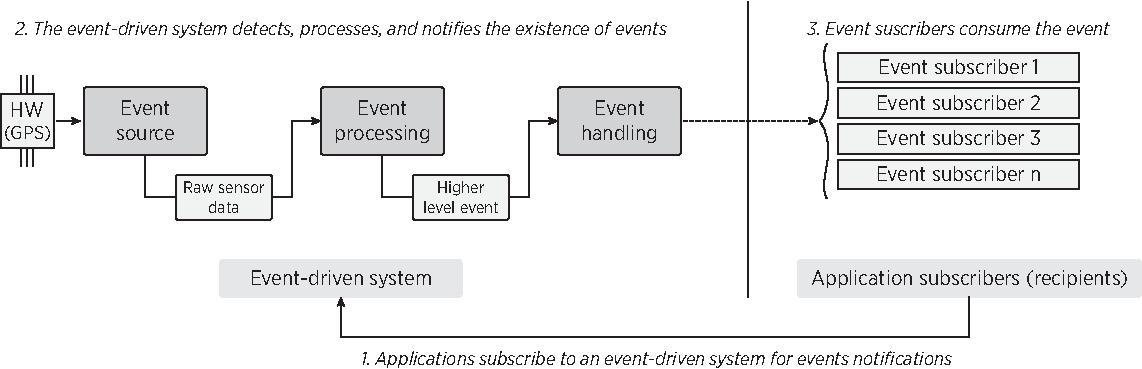
\includegraphics[width=0.3\textwidth]{images/event-driven-system.pdf}
  \end{tikzfigure} 
  }

  \block{Movimiento desde la perspectiva de la física}{
  \begin{tikzfigure}[Componentes de un sistema dirigido por eventos]
  %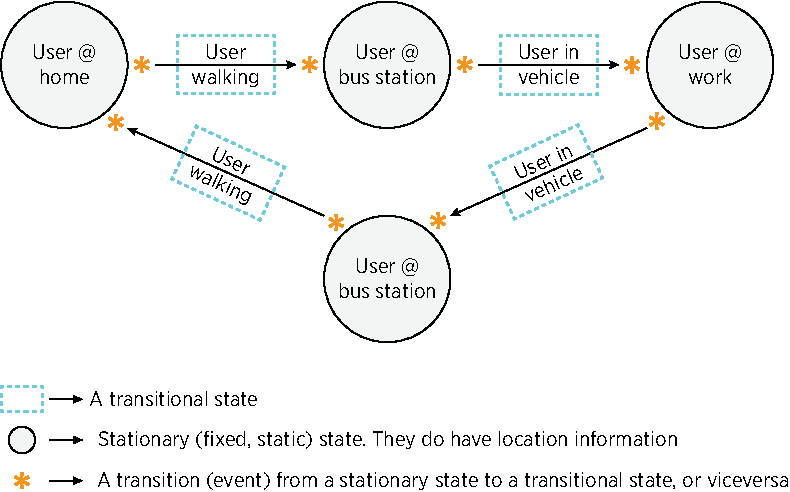
\includegraphics[width=0.25\textwidth]{images/physics-perspective-of-motion}
  Figura o mapa de stay points | Gráfica velocidad vs tiempo (valores estables = stay point))
  \end{tikzfigure}
  }

  \block{Sistemas dinámicos cognitivos}{
  \begin{tikzfigure}[Sistemas dinámicos cognitivos]
  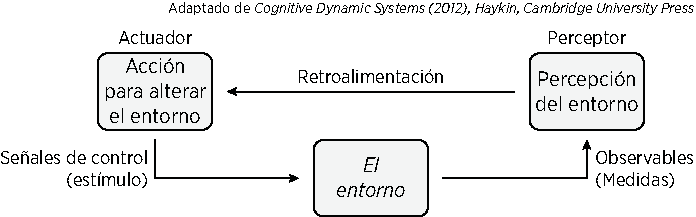
\includegraphics[width=0.25\textwidth]{images/cognitive-dynamic-systems.pdf}
  \end{tikzfigure}  
  }

\column{0.5}
  \block{Solución Propuesta}{
    \begin{tikzfigure}[Arquitectura de la solución propuesta]
    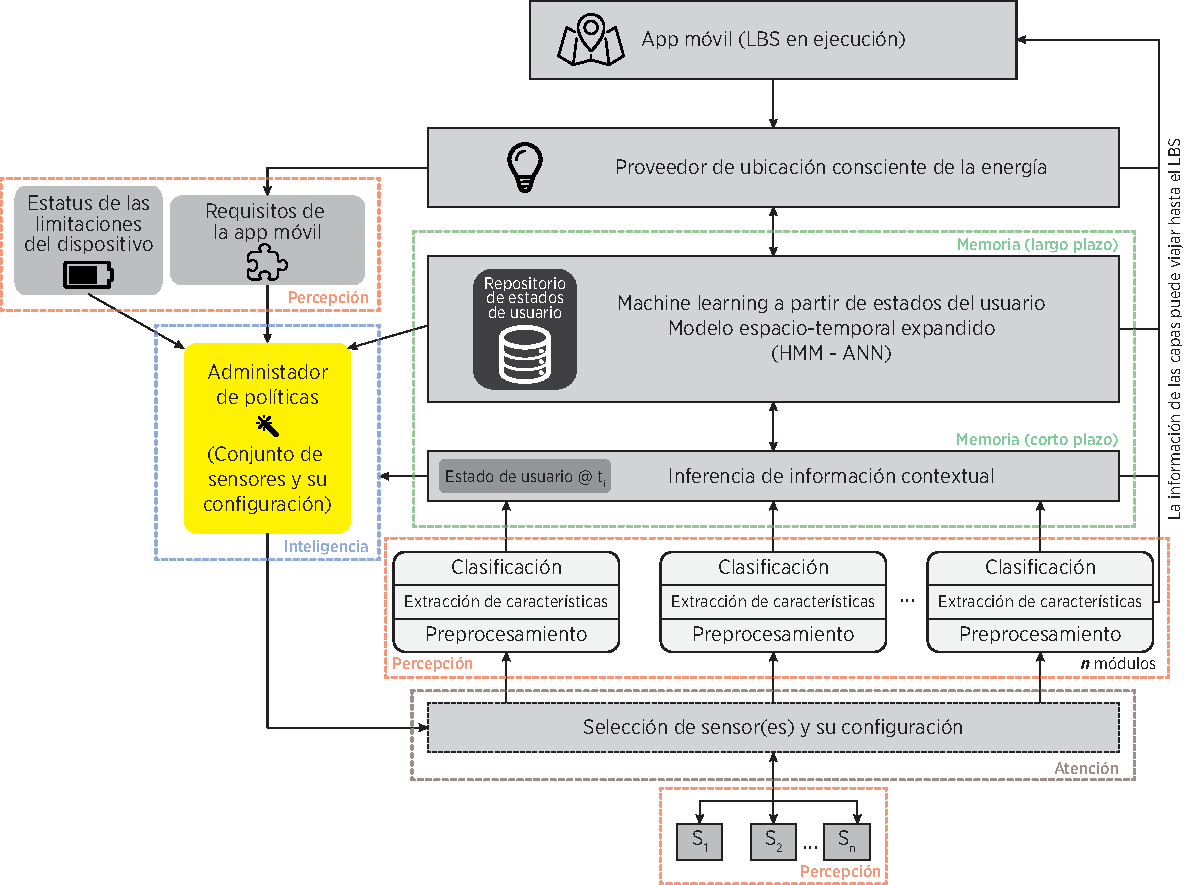
\includegraphics[width=0.4\textwidth]{images/solution-general-overview.pdf}
    \end{tikzfigure}

    \begin{tikzfigure}[Modelo espacio-temporal expandido de la solución propuesta]
    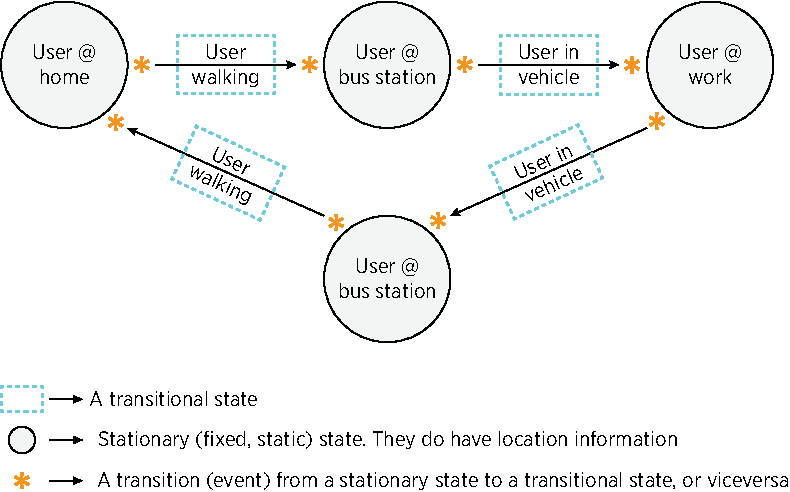
\includegraphics[width=0.3\textwidth]{images/zoom-spatial-time-model.pdf}
    \end{tikzfigure}
}

\end{columns}

\block{Resultados preliminares}{
\Large
\begin{itemize}
  \item Posibilidad de detectar puntos de interés en el smartphone validada
  \item Detección de actividad del usuario en base al acelerómetro verificada
\end{itemize}
  %\innerblock{H}{C}
  %\coloredbox{Contnt} 
}

\end{document}